\documentclass{article}
\usepackage{amsmath}
\usepackage{tikz}
\usepackage{hyperref}
\usetikzlibrary{positioning}
\newcommand\abs[1]{\left|#1\right|}

\begin{document}

\title{%
  Introduction to Graph Theory \\
  \large by Richard Trudeau \\
   Ch. 2 Solutions}
   \author{Tyler Bailey}
\maketitle

\begin{enumerate}
\item[1] List all subsets of the set $\{1, 2, 3\}$. There are 8 of them.

\textbf{Solution:} $\emptyset, \{1\}, \{2\}, \{3\}, \{1, 2\}, \{2, 3\}, \{1, 3\}, \{1, 2, 3\}.$

\item[2] It follows from the Law of Excluded Middle that to prove a mathematical statement true, it suffices
to show that it cannot be false. Letting $A$ be a set and $j$ an empty set, show that the statement ``$j$ is a subset of $A$ cannot be false and so is true". This proves that an empty set is a subset of every set.

\textbf{Solution:} This is vacuously true. Implications are true whenever the antecedent is false. The antecedent is ``for all $x \in j$", of which there are no such $x$.

\item[3] This is another version of Russell's Paradox. The village barber shaves those and only those men who live in the village and do not shave themselves. The village barber is a man and lives in the village. Consider the question ``Who shaves the barber?" Then explain how this situation is equivalent to Russel's Paradox.

\textbf{Solution:} The book uses the terminology: `ordinary' sets have normal elements while `extraordinary' sets can have themselves as elements. Russell's Paradox: $S = \{A \mid A$ is an ordinary set$\}$. Now, $S$ contains only ordinary sets. If $S$ was ordinary, it would contain itself and therefore be extraordinary. If $S$ was extraordinary, it would not be an element of itself since it only contains ordinary elements.

Current problem: If the barber shaves himself, then he is not in the set, because only men who do not shave themselves are in the set. If the barber does not shave himself, he is in the set. But then the barber would be shaving himself, which is another contradiction. This is equivalent to the paradox because the only two possible situations are in fact impossible.

\item[4] Let $S$ be the collection of all sets that can be described in an English sentence of twenty-five words or less. Is $S$ a set? Why or why not?

\textbf{Solution:} No, $S$ is not a set. We can recast Russell's Paradox in 25 or less words (in fact it is above).

\item[5] If $v$ is an integer greater than or equal to $2$, the \textbf{path graph} on $v$ vertices, denoted $P_v$, is the graph having vertex set $\{1, 2, 3, \ldots, v\}$ and the edge set $\{ \{1, 2\}, \{2, 3\}, \{3, 4\}, \ldots, \{v - 1, v\} \}$. Draw the first five path graphs. The find and prove a formula for the number of edges of $P_v$.

\textbf{Solution:}

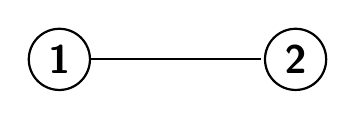
\begin{tikzpicture}[shorten >=1pt,auto,node distance=3cm,
                    thick,main node/.style={circle,draw,font=\sffamily\Large\bfseries}]

  \node[main node] (1) {1};
  \node[main node] (2) [right of=1] {2};

  \path[every node/.style={font=\sffamily\small}]
    (1) edge node [left] {} (2);
\end{tikzpicture}

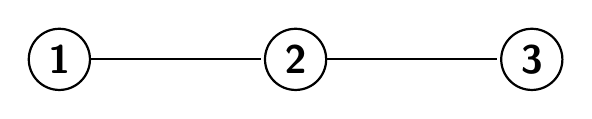
\begin{tikzpicture}[shorten >=1pt,auto,node distance=3cm,
                    thick,main node/.style={circle,draw,font=\sffamily\Large\bfseries}]
                    
  \node[main node] (1) {1};
  \node[main node] (2) [right of=1] {2};
  \node[main node] (3) [right of=2] {3};

  \path[every node/.style={font=\sffamily\small}]
    (1) edge node [left] {} (2)
    (2) edge node [right] {} (3);
\end{tikzpicture}
$\ldots$ etc.

The formula for the number of edges of $P_v$ is $v - 1$ and this can be proved by starting at $\abs{v} = 2$ where $\abs{e} = 1$ and in the induction step by noticing each time we add a new vertex we add one more edge.

\item[6] If $v$ is an integer greater than or equal to 4, the $\textbf{wheel graph}$ on $v$ vertices, denoted $W_v$, is the graph having vertex set $\{1, 2, 3, \ldots, v\}$ and edge set $\{ \{1, 2\}, \{1, 3\}, \ldots, \{1, v\}, \{2, 3\}, \{3, 4\}, ... \{v - 1, v\}, \{v, 2\} \}$. Draw the first $5$ wheel graphs. Then find and prove a formula for the number of edges of $W_v$.

\textbf{Solution: }

\begin{tikzpicture}[shorten >=1pt,auto,node distance=3cm,
                    thick,main node/.style={circle,draw,font=\sffamily\Large\bfseries}]
                    
  \node[main node] (4) {4};
  \node[main node] (2) [right=3cm of 1] {2};
  \node[main node] (3) [below=3cm of 1] {3};
  \node[main node] (1) [below right=0.75cm and 0.75cm of 1] {1};

  \path[every node/.style={font=\sffamily\small}]
    (1)	edge node [left] {} (2)
    		edge node [left] {} (3)
    		edge node [left] {} (4)
    (2)	edge node [right] {} (3)
    (3)	edge node [right] {} (4)
    (4)	edge node [right] {} (2);

\end{tikzpicture}

\begin{tikzpicture}[shorten >=1pt,auto,node distance=3cm,
                    thick,main node/.style={circle,draw,font=\sffamily\Large\bfseries}]
                    
  \node[main node] (1) [below left=1.25cm and 1.25cm of 2] {1};
  \node[main node] (2) {2};
  \node[main node] (3) [below=3cm of 2] {3};
  \node[main node] (5) [right=3cm of 2] {5};
  \node[main node] (4) [right=3cm of 3] {4};

  \path[every node/.style={font=\sffamily\small}]
    (1)	edge node [left] {} (2)
    		edge node [left] {} (3)
    		edge node [left] {} (4)
    		edge node [left] {} (5)
    (2)	edge node [right] {} (3)
    (3)	edge node [right] {} (4)
    (4)	edge node [right] {} (5)
    (5)	edge node [right] {} (2);

\end{tikzpicture}

$\ldots$ etc.

For $W_v$ we have $\abs{e} = 2(v-1)$. This can again be proved by induction, and in the inductive step by noting that if we add a new vertex, we add three new edges and remove one edge, namely we add the edges connecting the new vertex to $1$, the new vertex to $v - 1$, and the new vertex to $2$, and remove the edge from $v - 1$ to $2$.

Alternatively, we can just read it off from the edge set description. There are $v - 1$ edges connected to 1, $v - 2$ edges connecting $2$ to $3$, $3$ to $4$... etc, and $1$ edge connecting $v$ to $2$ for a total of $2(v - 1)$ edges.

\item[7] Using the fact that the number of edges of $K_v$ is $\frac{1}{2}v(v-1)$, prove that $1 + 2 + \ldots + (v - 1) = \frac{1}{2}v(v-1)$ for any integer $v \geq 2$. Do not use any arithmetic or algebra.

\textbf{Solution:} The number of unique edges connected to the first vertex of $K_v$ is $v - 1$ since it is connected to every vertex (but not itself). The next vertex is connected to $v - 2$ unique vertices (not itself, and not the first vertex) etc, until we get to the node which only has $1$ unique edge remaining.

\item[8] Let $G$ be a graph with $v$ vertices and $e$ edges. In terms of $v$ and $e$, how many edges has $\overline{G}$?

\textbf{Solution:} $e_G + e_{\overline{G}} = \frac{1}{2}v(v-1) \implies e_{\overline{G}} = \frac{1}{2}v(v-1) - e_G$.

\item[9] Prove: if $G$ has $v = 6$ then $G$ or $\overline{G}$ (possibly both) has a subgraph isomorphic to $K_3$.

\textbf{Solution:} A vertex of $v$ of $G$ has $\geq 3$ neighbors or $\geq 3$ non-neighbors by the pigeonhole principle.
\begin{enumerate}
	\item{Case 1:} If $v$ has $\geq 3$ neighbors and any pair of the $3$ neighbors $x, y, z$ are adjacent to each other (WLOG $x$, $y$), then $vxy \cong K_3$. If none of $x, y, z$ are adjacent to each other, then $xyz \cong K_3$.
    \item{Case 2:} If $v$ has $\geq 3$ non-neighbors and any pair of the three $x, y, z$ are non-neighbors (WLOG $x$, $y$), then $vxy \cong K_3$. If no two of $x, y, z$ are non-neighbors then $xyz \cong K_3$.
\end{enumerate}

\item[10] Use Exercise 9 to prove that in any gathering of six people there are either 3 people who are mutually acquainted or three people who are mutually unacquainted, possibly both.

\textbf{Solution:} Let $G$ be a graph where a vertex represents a person and an edge represents them being acquainted. Then, in $\overline{G}$, an edge represents them being not acquainted. Exercise 9 implies $G$ or $\overline{G}$ has a subgraph isomorphic to $K_3$, so either $3$ people know each other, $3$ people don't, or possibly both.

\item[11] Prove: the sum of degrees of the vertices of a graph is $2e$.

\textbf{Solution:} Just note that every edge must touch two vertices. Alternatively, considered the set of ordered pairs $P = \{(v, e) \mid v$ has an edge $e\}$. The number of items with vertex $v$ in the set will be $\mathrm{deg}{v}$ so we have $\abs{P} = \sum_v{\mathrm{deg}(v)}$. On the other hand, as mentioned above, each $e$ will appear twice in $P$ so $\abs{P} = \sum_e{2} = 2e$.

\item[12] Use exercise 11 to answer these questions:
\begin{enumerate}
	\item If a graph has $v = 9, 4$ vertices of degree $3$, $2$ vertices of degree $5$, $2$ of degree $6$ and 1 of degree 8, how many edges has the graph?
	\item $UG$ has $v = 6$, and every vertex has degree $3$; prove that there are however no graphs with $v = 7$ in which every vertex has degree 3.
\end{enumerate}
\textbf{Solution:}
\begin{enumerate}
	\item $\sum\mathrm{deg}(v) = 4 \cdot 3 + 2 \cdot 5 + 2 \cdot 6 + 1 \cdot 8 = 42 \implies e = 21$.
	\item $\sum\mathrm{deg}(v) = 7 \cdot 3 = 21 \neq 2e$.
\end{enumerate}

\item[13] Prove that $C_5 \cong \overline{C_5}$.

\textbf{Solution:} Move vertices 5 and 2 in $\overline{C_5}$ to get the familiar graph.

$C_5$

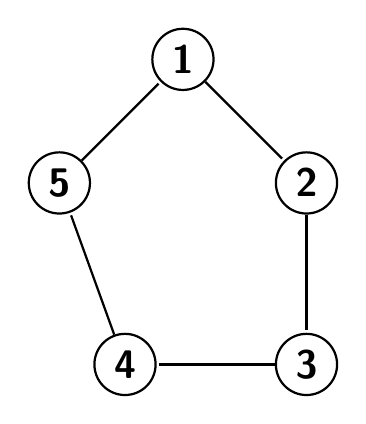
\begin{tikzpicture}[shorten >=1pt,auto,node distance=3cm,
                    thick,main node/.style={circle,draw,font=\sffamily\Large\bfseries}]
                    
  \node[main node] (1) {1};
  \node[main node] (2) [below right=1cm and 1cm of 1] {2};
  \node[main node] (3) [below=1.5cm of 2] {3};
  \node[main node] (4) [left=1.5cm of 3] {4};
  \node[main node] (5) [below left=1cm and 1cm of 1] {5};

  \path[every node/.style={font=\sffamily\small}]
    (1)	edge node [left] {} (2)
    (2)	edge node [right] {} (3)
    (3)	edge node [right] {} (4)
    (4)	edge node [right] {} (5)
    (5)	edge node [right] {} (1);

\end{tikzpicture}

$\overline{C_5}$

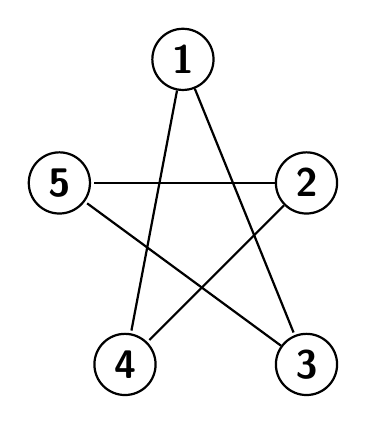
\begin{tikzpicture}[shorten >=1pt,auto,node distance=3cm,
                    thick,main node/.style={circle,draw,font=\sffamily\Large\bfseries}]
  \node[main node] (1) {1};
  \node[main node] (2) [below right=1cm and 1cm of 1] {2};
  \node[main node] (3) [below=1.5cm of 2] {3};
  \node[main node] (4) [left=1.5cm of 3] {4};
  \node[main node] (5) [below left=1cm and 1cm of 1] {5};

  \path[every node/.style={font=\sffamily\small}]
    (1)	edge node [left] {} (3)
    		edge node [left] {} (4)
    (2)	edge node [right] {} (4)
    		edge node [right] {} (5)
    (3)	edge node [right] {} (5);

\end{tikzpicture}

$\overline{C_5}$

\begin{tikzpicture}[shorten >=1pt,auto,node distance=3cm,
                    thick,main node/.style={circle,draw,font=\sffamily\Large\bfseries}]
  \node[main node] (1) {1};
  \node[main node] (3) [below right=1cm and 1cm of 1] {3};
  \node[main node] (5) [below=1.5cm of 2] {5};
  \node[main node] (2) [left=1.5cm of 5] {2};
  \node[main node] (4) [below left=1cm and 1cm of 1] {4};

  \path[every node/.style={font=\sffamily\small}]
    (1)	edge node [left] {} (3)
    		edge node [left] {} (4)
    (2)	edge node [right] {} (4)
    		edge node [right] {} (5)
    (3)	edge node [right] {} (5);

\end{tikzpicture}

To prove that no other cyclic graph is equal to its complement, we use the fact that $G \cong \overline{G} \implies e_G = e_{\overline{G}}$ and $e_G = v$ for cyclic graphs. Therefore:

\begin{align}
e_G + e_{\overline{G}} = 2v &\implies 2v = \frac{1}{2}v(v - 1) \\
	&\implies 0 = v^2 - 5v \\
	&\implies 0 = v(v - 5)
\end{align}
The only solutions are $v = 0, 5$ so there can be no other cyclic graphs that are equal to their complement.

\item[14] Prove that if $G \cong \overline{G}$ then $v$ or $v - 1$ is a multiple of 4. You might use the number of edges of $K_v$ and that fact that isomorphic graphs have the same number of edges.

\textbf{Solution:} Suppose $G \cong \overline{G}$ and $G$ has $v$ vertices. We know $e_G = e_{\overline{G}}$ and that $e_G + e_{\overline{G}} = \frac{1}{2}v(v - 1)$, so:
\begin{align}
e_G + e_{\overline{G}} = 2e_G &\implies 2e_G = \frac{1}{2}v(v - 1) \\
	&\implies 4e_G = v(v - 1)\\
\end{align}
So either $v$ or $v - 1$ must divide 4, because it is not possible that they both divide 2.

\item[15] If $G \cong \overline{G}$, $G$ is called a \textbf{self-complementary graph}. Exercise 13 says that $C_5$ is self-complementary and is the only cyclic graph that is. Find two other self-complementary graphs.

\textbf{Solution:}

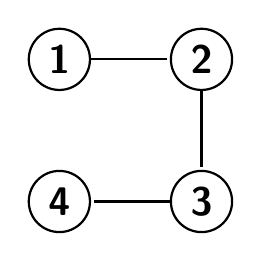
\begin{tikzpicture}[shorten >=1pt,auto,node distance=3cm,
                    thick,main node/.style={circle,draw,font=\sffamily\Large\bfseries}]
  \node[main node] (1) {1};
  \node[main node] (2) [right=1cm of 1] {2};
  \node[main node] (3) [below=1cm of 2] {3};
  \node[main node] (4) [left=1cm of 3] {4};

  \path[every node/.style={font=\sffamily\small}]
    (1)	edge node [left] {} (2)
    (2)	edge node [right] {} (3)
    (3)	edge node [right] {} (4);
\end{tikzpicture}

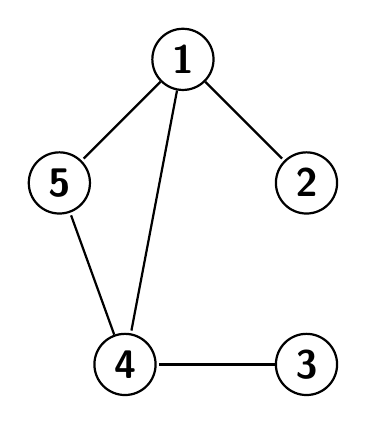
\begin{tikzpicture}[shorten >=1pt,auto,node distance=3cm,
                    thick,main node/.style={circle,draw,font=\sffamily\Large\bfseries}]
  \node[main node] (1) {1};
  \node[main node] (2) [below right=1cm and 1cm of 1] {2};
  \node[main node] (3) [below=1.5cm of 2] {3};
  \node[main node] (4) [left=1.5cm of 3] {4};
  \node[main node] (5) [below left=1cm and 1cm of 1] {5};

  \path[every node/.style={font=\sffamily\small}]
    (1)	edge node [left] {} (2)
    		edge node [left] {} (5)
    		edge node [left] {} (4)
    (3)	edge node [right] {} (4)
    (4)	edge node [right] {} (5);

\end{tikzpicture}

\item[16] Find a self-complementary graph with $v = 8$

\textbf{Solution:} These are in the back of the book.

\item[17] Since there are an odd number of graphs having $v = 4$, one of them must be complementary. Which one?

\textbf{Solution:} See example from solution 15.

\item[18] How many different correspondences are there between two sets with 10 unique elements?

\textbf{Solution:} $10!$. For a bijection to occur, there must be an invertible mapping. Mapping the first element gives 10 possibilities, mapping the next element gives 9, ...

\item[19] Put $\{1, 2, 3, \cdots\}$ and $\{2, 4, 6, \cdots\}$ into a one-to-one correspondence.

\textbf{Solution:} Multiplication and division by 2 give this bijection.

\item[20] Use the fact that if two graphs are isomorphic then for any subgraph there is an isomorphic subgraph to prove that the graphs in Figure 35 are not isomorphic.

\textbf{Solution:} Look at the subgraph $ACDEFG$. There $C$ and $E$ are adjacent vertices with $\mathrm{deg}(v) = 3$. There is no such subgraph in the other graph.

\item[21] $K_3$ with its vertices labeled has 17 unequal subgraphs. Draw them.

\textbf{Solution:} There are too many to draw here, but there are 3 graphs with single vertices, 3 graphs with two vertices, 1 graph with 3 vertices, 3 graphs with 2 vertices 1 edge, 3 graphs with 3 vertices 1 edge, 3 graphs with 3 vertices 2 edges, 1 graph with 3 vertices 3 edges, so 17 total.

\item[22] The number of non-isomorphic graphs of $K_3$ is only 7. Draw them.

\textbf{Solution:} Again, too many to draw, but just take one representative from each group in the previous problem.

\item[23] The graphs of Figure 46 are not isomorphic. Prove this by finding a subgraph of one that is not a subgraph of the other.

\textbf{Solution:} The graph on the right does not have a subgraph isomorphic to $K_3$.

\item[24] Satisfy yourself that isomorphic graphs have isomorphic complements and that consequently non-isomorphic graphs have non-isomorphic complements. Then use this fact to devise a proof that the graphs of Figure 31 are not isomorphic.

\textbf{Solution:} The graph on the LHS has 2 vertices with no edges while the graph on the RHS has 3.

\item[25] Use the technique of Exercise 24 to prove that the graphs of Figure 46 are not isomorphic.

\textbf{Solution:} The LHS's complement is isomorphic to $C_6$ while the RHS's complement is isomorphic to two disjoint $K_3$ graphs.

\item[26] Draw all graphs having $v = 5$. There are 34 of them.

\textbf{Solution:} There are too many for me to have here, but see e.g. this link: \url{http://www.graphclasses.org/smallgraphs.html#nodes5}

\item[27] In the table on page 54, the numbers in the second column are mostly even. If we ignore the first row on the gorund that $v = 1$ is such a trivial situation that its uniqueness is unremarkable, that leaves $v = 4$ as the only number of vertices listed for which there are an odd number of graphs. Do you think this is due to chance, or can you think of some reason why $v = 4$ should be unique? If the table were continued, do you think more odd numbers would turn up in the second column?

\textbf{Solution:} I am guessing there $v = 4$ is special and that there will be few if any odd numbers further down the last. That being said, I am not sure why that is the case. It seems like the only case where it would be possible to have an odd number in the table is if there is an odd number of self-complementary graphs.

\item[28] Prove that the graphs from Figure 47 are isomorphic.

\textbf{Solution:} If we label the figure on the LHS by starting with 1 at the apex and continuing clockwise, then the reordering the vertices on the page by $(1, 2, 3, 4, 5, 6, 7) \mapsto (1, 3, 5, 7, 2, 4, 7)$ allows us to have the graph on the RHS.

\item[29] Prove that the graphs of Figure 48 are all isomorphic to the utility graph.

\textbf{Solution:} I will give the vertex mappings that can allow us to rearrange the graph on the page to the utility graph.
\begin{enumerate}
\item[a] Numbering from the top left, counter-clockwise, $(1, 2, 3, 4, 5, 6) \mapsto (1, 3, 5, 6, 4, 2)$.
\item[b] Numbering the outside triangle $(1, 2, 3)$ and the inner vertical graph $(4, 5, 6)$ gives us the rearrangement $(1, 5, 6, 4, 3, 2)$.
\item[c] $(1, 2, 3, 4, 5, 6) \mapsto (1, 3, 5, 6, 4, 2)$.
\end{enumerate}

\item[30 - 37] In each of Figures 49 - 56, decide whether or not the two are isomorphic.

\textbf{Solution:} The answers to this are in the back of the book. None of them are particularly difficult, so just be persistent.

\item[38] A chess tournament consists of 25 players, each of whom plays one game with every other player. How many games are played during this tournament?

\textbf{Solution:} This question is asking how many edges are in the graph $K_{25}$, so the answer is 300.

\item[39] When I said on page 56 ``There is no simple way of determining the number of graphs given $v$," I meant of course that there is no simple way of determining the number of non-isomorphic graphs having a given $v$. Prove that there are exactly $2^{\frac{1}{2}v(v-1)}$ unequal graphs whose $v$ vertices have been labeled with the integers from 1 to $v$.

\textbf{Solution:} We know there are $\frac{1}{2}v(v-1)$ potential edges in every graph. So, we can enumerate every possible graph by going through each of the $v$ vertices and deciding whether there is an edge of not. Every choice has two possibilities, so we have $2^{\frac{1}{2}v(v-1)}$ total decisions, every one leading a unique graph.

\end{enumerate}

\end{document}